\documentclass[a4paper, 11pt]{article}
\usepackage[cuestionario=3]{estilo}

\begin{document}

    \maketitle

    \section{Ejercicios}


      \begin{ejercicio}
          Consider los conjuntos de hipótesis $\mathcal{H}_1$ y $\mathcal{H}_{100}$ que contienen funciones booleanas sobre 10 variables Booleanas, es decir $\mathcal{X} =\{-1,+1\}^{10}$. $\mathcal{H}_1$ contiene todas las funciones Booleanas que toman valor $+1$ en un único punto de $\mathcal{X}$ y $-1$ en el resto. $\mathcal{H}_{100}$ contiene todas las funciones Booleanas que toman valor $+1$ en exactamente 100 puntos de $\mathcal{X}$ y $-1$ en el resto.
          \begin{enumerate}
          \item ¿Cuántas hipótesis contienen $\mathcal{H}_1$ y $\mathcal{H}_{100}$ ?
          \item ¿Cuántos bits son necesarios para especificar una de las hipótesis en $\mathcal{H}_1$?
          \item ¿Cuántos bits son necesarios para especificar una de las hipótesis en $\mathcal{H}_{100}$?
          \end{enumerate}
          Argumente sobre la relación entre  la complejidad de una clase de funciones y la complejidad de sus componentes.
      \end{ejercicio}

      \begin{solucion}
          \begin{enumerate}
              \item $\mathcal{H}_1$ asigna 1 a un único punto de la muestra y -1 a todos los demás, luego en $\mathcal{H}_1$ hay tantas funciones diferentes como puntos haya en la muestra. Pero el espacio muestral $\mathcal{X}$ está compuesto por $2^{10} = 1024$ puntos diferentes, luego $\vert\mathcal{H}_1\vert = 1024$.

              Por otro lado, $\mathcal{H}_{100}$ está definida en función a su comportamiento sobre subconjuntos de $\mathcal{X}$ de tamaño 100; es decir, en esa clase hay tantas funciones como subconjuntos diferentes de tamaño 100 haya en $\mathcal{X}$. El número de formas de escoger $k$ elementos a partir de un conjunto de tamaño $n$ es conocido, se llama coeficiente binomial y vale lo siguiente:
              \[\begin{pmatrix}
                  n \\
                  k
              \end{pmatrix} = \frac{n!}{k!(n-k)!}
              \]
              Por tanto, el número de hipótesis contenidas en $\mathcal{H}_{100}$ es de $\vert\mathcal{H}_{100}\vert = \begin{pmatrix}
                  1024 \\
                  100
              \end{pmatrix} = \frac{1024!}{100!(1024-100)!} = 774662466804345233634010032024656517236965647168803935408596916906303252199494470709880165045781515893999614469740109324589034524935408592640$
              Hemos dejado que el número, de 141 cifras, se salga físicamente de la página para tener una idea de su magnitud.

              \item Para especificar una de las hipótesis en $\mathcal{H}_1$ basta indicar qué punto de la muestra tiene valoración positiva. Basta almacenar un número entre 1 y 1024, con lo que necesitamos $log_2(1024) = 10$ bits.

              \item Para especificar una de las hipótesis en $\mathcal{H}_{100}$ hay que indicar qué 100 puntos de la muestra tienen valoración positiva. Tenemos que almacenar 100 números que se mueven entre 1 y 1024, luego necesitamos $10\cdot10 = 100$ bits.
          \end{enumerate}

          En este estudio se aprecia cómo la complejidad de una clase de funciones no tiene por qué reflejar la complejidad de sus componentes; es decir, que una clase de funciones sea altamente compleja ---su cardinal sea muy elevado--- no quiere decir que, independientemente, las funciones miembro sean altamente complejas.

          Midiendo la complejidad en bits se ve claro: mientras que para representar funciones de $\mathcal{H}_{100}$ necesitamos 10 veces el número de bits que necesitan las representaciones de los miembros de $\mathcal{H}_1$, la clase $\mathcal{H}_{100}$ alberga del orden de $10^{141-3} = 10^{138}$ elementos más que la clase $\mathcal{H}_1$.

      \begin{ejercicio}
          Suponga que durante 5 semanas seguidas, recibe un correo postal que predice el resultado del partido de futbol del domingo, donde hay apuestas substanciosas. Cada lunes revisa la predicción y observa que la predicción es correcta en todas las ocasiones. El día de después del quinto partido recibe una carta diciendole que si desea conocer la predicción de la semana que viene debe pagar 50.000€. ¿Pagaría?
          \begin{enumerate}
              \item ¿Cuántas son las posibles predicciones gana-pierde para los cinco partidos?
              \item Si el remitente desea estar seguro de que al menos una persona recibe de él la predicción correcta sobre los 5 partidos, ¿cuál es el mínimo número de cartas que deberá de enviar?
              \item Después de la primera carta prediciendo el resultado del primer partido, ¿a cuantos de los seleccionados inicialmente deberá de enviarle la segunda carta?
              \item ¿Cuántas cartas en total se habrán enviado depués de las primeras cinco semanas?
              \item Si el coste de imprimir y enviar las cartas es de 0.5€ por carta, ¿Cuanto ingresa el remitente si el receptor de las 5 predicciones acertadas decide pagar los 50.000€?
              \item ¿Puede relacionar esta situación con la función de crecimiento y la credibilidad del ajuste de los datos?
          \end{enumerate}
      \end{ejercicio}

      \begin{solucion}
          \begin{enumerate}
              \item En cada partido hay dos posibles predicciones: gana o pierde. En los cinco partidos habrá, por tanto, $2^5  = 32$ posibles predicciones.
              \item La primera aproximación a esta pregunta es clara: necesitamos enviar al menos 32 predicciones y en cada predicción debemos usar 5 cartas, luego el número total de cartas enviadas debe ser al menos $32\cdot5 = 160$.

              Sin embargo, este no es el mínimo necesario, ya que las predicciones que resultan erróneas en el proceso deben descartarse; es decir: la primera semana debe enviar 32 cartas ---para poder cubrir al final las 32 predicciones necesarias---, la mitad de ellas prediciendo la victoria y la otra mitad prediciendo la derrota. Tras conocerse el resultado de la primera semana, habrá 16 destinatarios cuya predicción será incorrecta, así que a la semana siguiente sólo debe enviar 16 cartas ---a aquellos cuya primera predicción fue correcta---. Siguiendo este proceso, tras cinco semanas debe enviar, al menos, el siguiente número de cartas:
              \[
              32 + 16 + 8 + 4 + 2 = 62
              \]
              \item Como se ha indicado en el anterior apartado, basta enviarle la carta a la mitad de los seleccionados inicialmente; en particular, a aquellos cuya carta terminó conteniendo una predicción correcta.
              \item Como se ha indicado en el apartado 2, se habrán enviado 62 cartas.
              \item Si decide enviar sólo las 62 cartas necesarias y el receptor de la predicción acertada decide pagar el dinero, el ingreso es de $
              50000 - 62\cdot0.5 = 49969$ euros.
              \item Si vemos la estafa descrita en los apartados anteriores como un proceso de aprendizaje sobre el conjunto de $N$ partidos, y lo analizamos desde el punto de vista del estafador, tiene la función de crecimiento máxima ---es decir, $2^N$--- ya que puede implementar todas y cada una de las posibles predicciones. Aun sin conocer los resultados cada semana se podría conseguir la máxima función de crecimiento, ya que hemos visto que con al menos $N2^N$ cartas cubrimos todas las predicciones. Como la complejidad de nuestra clase de hipótesis es la más grande posible, sabemos que la credibilidad del ajuste de los datos es nula: podemos abarcarlos todos y un eventual acierto en la predicción tiene un valor extremadamente bajo. De hecho, cualquier dato futuro tendrá una probabilidad del 50\% de ser predicho, tal y como lo eran al principio. La generalización de este proceso es evidentemente nula, y se aprecia bien que la estafa se basa en que la capacidad de ajuste a los datos de entrenamiento no tiene por qué tener que generalizarse a los datos de test.

              Por otro lado, desde el punto de vista del receptor de las cartas parece que la función de crecimiento es 1, ya que sólo conoce las cartas que él recibió; esto le permite dar mucho valor a la credibilidad del método, ya que con una clase de hipótesis tan simple ---según su punto de vista--- se consigue un sorprendente ajuste a los resultados.
          \end{enumerate}
      \end{solucion}


      \begin{ejercicio}
        En un experimento para determinar la distribución del tamaño de los peces en un lago, se decide echar una red para capturar una muestra representativa. Así se hace y se obtiene una muestra suficientemente grande de la que se pueden obtener conclusiones estadísticas sobre los peces del lago. Se obtiene la distribución de peces por tamaño y se entregan las conclusiones. Discuta si las conclusiones obtenidas servirán para el objetivo que se persigue e identifique si hay que lo impida.
      \end{ejercicio}

      \begin{solucion}
          En el estudio teórico del aprendizaje automático se presupone casi siempre un escenario muy general, pero las pocas hipótesis necesarias para demostrar los resultados son cruciales. Si estas no se cumplen, el estudio generado no tiene por qué cumplir con lo esperado y no podremos extraer unas conclusiones fiables.

          Una de las hipótesis más importantes en las cotas estadísticas, como la de Hoeffding y la de Vapnik–Chervonenkis, que determinan la bondad de las conclusiones, es que las muestras de entrenamiento y de test deben estar extraídas de una misma distribución.

          Esta hipótesis corre demasiado peligro en este ejemplo: si el lago es lo suficientemente grande, el tipo de peces extraídos con la red de una zona concreta puede no ser representativo de la distribución total del lago; si la red se echa una única vez y en un único lugar, el \textbf{sesgo muestral} será demasiado elevado como para concluir que el estudio de la muestra se puede extender a la distribución que se espera encontrar en todo el lago.
      \end{solucion}

      \begin{ejercicio}
        Considere la siguiente aproximación al aprendizaje. Mirando los datos, parece que los datos son linealmente separables, por tanto decidimos usar un simple perceptron y obtenemos un error de entrenamiento cero con los pesos óptimos encontrados. Ahora deseamos obtener algunas conclusiones sobre generalización, por tanto miramos el valor $d_{vc}$ de nuestro modelo y vemos que es $d+1$. Usamos dicho valor de $d_{vc}$ para obtener una cota del error de test.  Argumente a favor o en contra de esta forma de proceder identificando los posible fallos si los hubiera y en su caso cual hubiera sido la forma correcta de actuación.
      \end{ejercicio}

      \begin{solucion}
        El primer fallo evidente en este proceso es el haber obtenido información de la muestra antes de decidir el modelo para aproximarlos. El simple hecho de conocer la forma de la muestra de entrenamiento nos condiciona en la elección de un modelo para que ajuste esos datos y no la distribución general; nos acercamos así a una situación peligrosa que debemos evitar: el sobreajuste.

        Además se está cometiendo otro error grave: la elección del modelo está sesgada en vista a los datos de entrenamiento, luego la cota $d_{VC}$ es probablemente errónea; es la cota del modelo, pero no del modelo que sigue la distribución general. Así, el estudio sobre la generalización y la cota del error de test no nos sirven: su falta de rigor nos impide usarlas para extraer cualquier conclusión.

        La forma correcta de actuar en estos casos debe empezar por elegir el modelo de aprendizaje antes siquiera de haber visto los datos con los que contamos para entrenarlo. Podemos obtener información general del problema o del espacio en el que se va a trabajar, pero nunca de la muestra de entrenamiento.
      \end{solucion}

      \begin{ejercicio}
          Suponga que separamos 100 ejemplos de un conjunto $\mathcal{D}$ que no serán usados para entrenamiento sino que serán usados para seleccionar una de las tres hipótesis finales $g_1$, $g_2$ y $g_3$ producidas por tres algoritmos de aprendizaje distintos entrenados sobre el resto de datos. Cada algoritmo trabaja con un conjunto $\mathcal{H}$ de tamaño 500. Nuestro deseo es caracterizar la precisión de la estimación $E_{out}(g)$ sobre la hipótesis final seleccionada cuando usamos los mismos 100 ejemplos para hacer la estimación.
          \begin{enumerate}
          \item ¿Qué expresión usaría para calcular la precisión? Justifique la decisión
          \item ¿Cuál es el nivel de contaminación de estos 100 ejemplos comparándolo con el caso donde estas muestras fueran usadas en el entrenamiento en lugar de en la selección final?
          \end{enumerate}
      \end{ejercicio}

      \begin{solucion}
          \begin{enumerate}
              \item Queremos calcular una cota del error fuera de la muestra ---es decir, en los 100 ejemplos separados--- conociendo el error en la muestra de entrenamiento, y con un valor preciso del cardinal de la clase de funciones. Así, usaría la desigualdad de Hoeffding siguiente:
              \[
              \mathbb{P}[\vert E_{in}(g_i) - E_{out}(g_i)\vert > \epsilon] \leq 2Me^{-2\epsilon^2N}
              \]
              donde $M$ es 500, el tamaño de $\mathcal{H}$; $N$ es el tamaño de la muestra de entrenamiento y $\epsilon$ la precisión con la que queremos caracterizar la estimación.
              \item Si los 100 ejemplos fueran usados en el entrenamiento y luego tomados como muestra de test, estaríamos aprendiendo del test, contaminando así lo aprendido. El nivel de contaminación en este caso es mucho menor, ya que los obviamos hasta que hemos aprendido de los datos.
          \end{enumerate}
      \end{solucion}

      \begin{ejercicio}
          Considere la tarea de seleccionar una regla del vecino más cercano. ¿Qué hay de erróneo en la siguiente lógica que se aplica a la selección de k? ( Los límites son cuando $N\rightarrow\infty$ ). \emph{ Considere la posibilidad de establecer la clase de hipótesis $H_{NN}$ con $N$ reglas, las k-NN hipótesis, usando $k =1,\dots,N$. Use el error dentro de la muestra para elegir un valor de k que minimiza $E_{in}$. Utilizando el error de generalización para N hipótesis, obtenemos la conclusión de que $E_{in} \rightarrow E_{out}$ porque $\log N / N \rightarrow 0$. Por lo tanto concluimos que asintóticamente,  estaremos eligiendo el mejor valor de k, basadonos solo en $E_{in}$.}
      \end{ejercicio}


      \begin{solucion}
        ---
      \end{solucion}

      \begin{ejercicio}
          \begin{enumerate}
          \item Considere un núcleo Gaussiano en un modelo de base radial. ¿Que representa $g(x)$ (ecuación 6.2 del libro LfD) cuando $||x||\rightarrow \infty$ para el modelo RBF no-paramétrico versus el modelo RBF paramétrico, asumiendo los $\textbf{w}_n$ fijos.
          \item Sea $Z$ una matriz cuadrada de características definida por $Z_{nj}=\Phi_j(\textbf{x}_n)$ donde $\Phi_j(\textbf{x})$ representa una transformación no lineal. Suponer que $Z$ es invertible. Mostrar que  un modelo paramétrico de base radial, con $g(\textbf{x})=\textbf{w}^T\Phi(\textbf{x})$ y $\textbf{w}=Z^{-1}\textbf{y}$, interpola los puntos de forma exacta. Es decir, que $g(\textbf{x}_n)=\textbf{y}_n$, con $E_{in}(g)=0$.
          \item ¿Se verifica siempre que $E_{in}(g)=0$ en el modelo no-paramétrico?
          \end{enumerate}
      \end{ejercicio}

      \begin{solucion}
        ---
      \end{solucion}

      \begin{ejercicio}
        Verificar que la función $\mathrm{sign}$ puede ser aproximada por la función $\tanh$. Dado $\textbf{w}_1$ y $\epsilon>0$ encontrar $\textbf{w}_2$ tal que $\vert\mathrm{sign}(\textbf{x}_n^T \textbf{w}_1) - \tanh(\textbf{x}_n^T\textbf{w}_2)\vert \leq \epsilon$ para $\textbf{x}_n\in \mathcal{D}$ (Ayuda: analizar la función $\tanh(\alpha\textbf{x}),\, \alpha\in$ R)
      \end{ejercicio}

      \begin{solucion}
          En la Figura \ref{img:tanh} podemos comprobar visualmente que la función $\operatorname{tanh}(\alpha x)$ converge a la función signo cuando hacemos crecer $\alpha$.

          Se ve claro cómo el parámetro $\alpha$ mide, de alguna manera, cuán inclinada está la pendiente que une las constantes -1 y 1 de forma continua, así que cuanto mayor sea, más aproximará la tangente hiperbólica a la función signo.

          \begin{figure}[!htb]
              \centering
              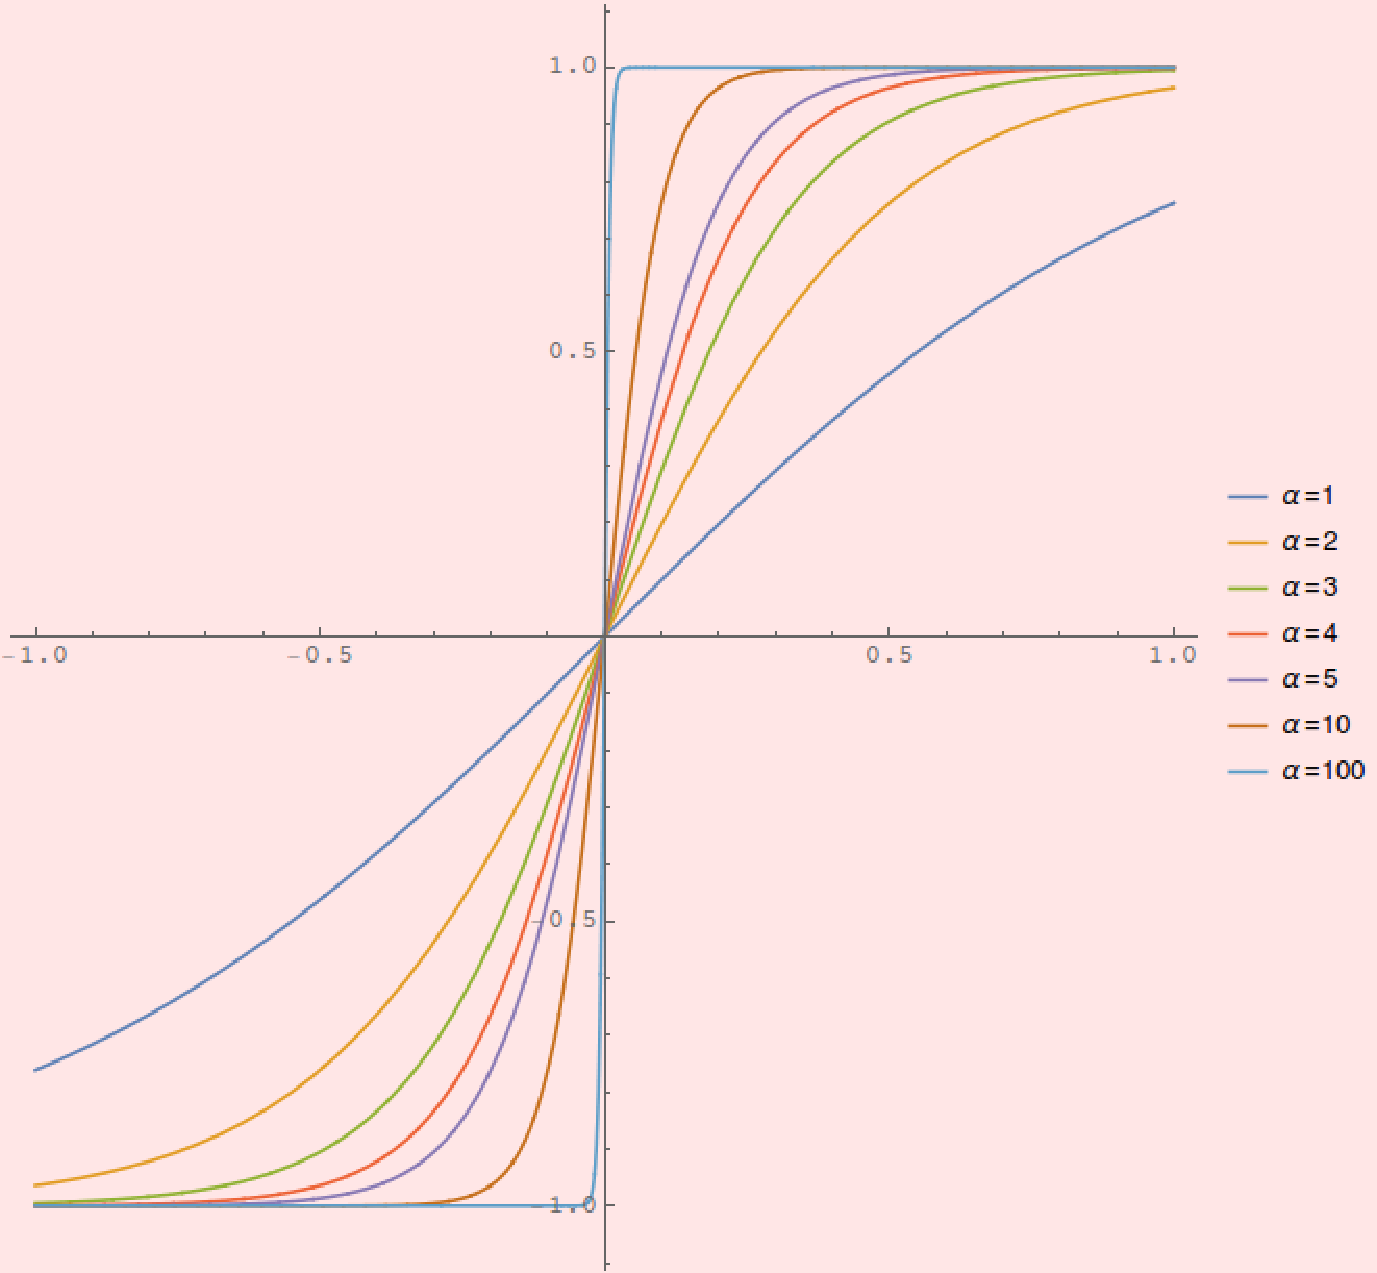
\includegraphics[scale=0.5]{tanh.pdf}
              \caption{Convergencia de la tangente hiperbólica a la función signo.}
              \label{img:tanh}
          \end{figure}

          Para verlo de una forma analítica basta estudiar los límites de la función tangente hiperbólica punto por punto:
          \begin{itemize}
              \item Sea $x = 0$. Entonces es claro que \[\lim_{\alpha\to\infty} tanh(\alpha x) = tanh(0) = 0 = sign(x)\]
              \item Sea $x > 0$ fijo. Entonces tenemos que \[\lim_{\alpha\to\infty} tanh(\alpha x) = \lim_{y\to+\infty} tanh(y) = 1 = sign(x)\]
              \item Sea $x < 0$ fijo. Entonces tenemos que \[\lim_{\alpha\to\infty} tanh(\alpha x) = \lim_{y\to-\infty} tanh(y) = -1 = sign(x)\]
          \end{itemize}
          Concluimos así que, fijado $x\in\mathbb{R}$:
          \[
          \lim_{\alpha\to\infty} tanh(\alpha x) = sign(x)
          \]

          La anterior igualdad nos dice que $\forall \epsilon>0$, existe un $\alpha \in \mathbb{R}$ tal que $\vert\mathrm{sign}(x) - \tanh(\alpha x)\vert \leq \epsilon$.

          Usando esta idea para responder al enunciado, podemos razonar como sigue:

          Fijado $\epsilon > 0$, existe un $\alpha \in \mathbb{R}$ tal que si definimos $w_2 = \alpha w_1$ ---es decir, el mismo vector de pesos $w_1$ pero con cada una de sus componentes multiplicadas por la constante $\alpha$---, podemos concluir que
          \begin{align*}
              \vert sign(x_n^Tw_1) - tanh(x_n^Tw_2) \vert &= \vert sign(x_n^Tw_1) - tanh(x_n^T\alpha w_1) \vert =\\
              &= \vert sign(x_n^Tw_1) - tanh(\alpha x_n^Tw_1) \vert = \\
              &= \vert sign(x) - tanh(\alpha x) \vert  \leq \epsilon
          \end{align*}
          donde al final hemos escrito $x := x_n^Tw_1$ para aclarar el uso del límite recién calculado.
      \end{solucion}

      \begin{ejercicio}
          Sea $V$ y $Q$ el número de nodos y pesos en una red neuronal,
          \[
          V=\sum_{l=0}^L d^{(l)}, \,\;\,
          Q=\sum_{l=1}^L d^{(l)}(d^{(l-1)}+1)
          \]
          En términos de $V$ y $Q$ ¿cuántas operaciones se realizan en un pase hacia adelante (sumas, multiplicaciones y evaluaciones de $\theta$)? ( Ayuda: analizar la complejidad en términos de $V$ y $Q$)
      \end{ejercicio}

      \begin{solucion}
        El cálculo de evaluaciones de $\theta$ es sencillo. Usando notación matricial, tenemos que la salida de la capa $\ell$ se calcula como:
        \[
        x^{(\ell)} = \begin{bmatrix}
            1\\
            \theta(s^{(\ell)})
        \end{bmatrix}
        \]
         donde $s^{(\ell)}$ es un vector de dimensión $d^{(\ell)}$. Es decir, la capa ${(\ell)}$ tiene que realizar $d^{(\ell)}$ evaluaciones de $\theta$. Ahora bien, la capa 0 es la de entrada, y no tiene cálculos de $\theta$, luego si llamamos $\vert\theta\vert$ al número total de evaluaciones de $\theta$ tenemos:
         \[
         \vert\theta\vert = 0 + d^{(1)} + d^{(2)} + \cdots + d^{(L)} = \sum_{\ell=1}^L d^{(\ell)} = V - d^{(0)}
         \]

         El número de sumas y multiplicaciones realizados en la capa ${(\ell)}$ está determinado por el número de sumas y multiplicaciones realizados en el cálculo de $s^{(\ell)}$, que es un vector cuya componente $j$-ésima viene determinada por la siguiente expresión:
         \[
         s_j^{(\ell)} = \sum_{i=0}^{d^{(\ell-1)}} w_{ij}^{(\ell)} x_i^{(\ell-1)}
         \]

         Cada componente $s^{(\ell)}$ de la entrada de la capa ${(\ell)}$ tiene por tanto $1 + d^{(\ell-1)}$ productos y $1 + d^{(\ell-1)}$ sumas ---nótese que la sumatoria empieza en cero---. Ahora bien, como $s^{(\ell)}$ es un vector de dimensión $d^{(\ell)}$, tenemos que tanto el número de sumas como el de multiplicaciones necesarias en la capa ${(\ell)}$, que notamos como $\vert\sigma\vert^{(\ell)}$ y $\vert\Pi\vert^{(\ell)}$, es de:
         \[
         \vert\sigma\vert^{(\ell)} = \vert\Pi\vert^{(\ell)} = d^{(\ell)}(1 + d^{(\ell-1)})
         \]

         El vector entrada $s^{(\ell)}$ debe calcularse en todas las capas menos en la capa $(0)$, luego concluimos que el número total de sumas, notado como  $\vert\sigma\vert$, es de:
         \begin{align*}
             \vert\sigma\vert &= 0 + d^{(1)}(1 + d^{(1-1)}) + d^{(2)}(1 + d^{(2-1)}) + \cdots + d^{(L)}(1 + d^{(L-1)}) = \\
             &= \sum_{\ell=1}^L d^{(\ell)}(1 + d^{(\ell-1)}) = Q
         \end{align*}

         De forma completamente análoga se concluye que el número total de multiplicaciones, notado como $\vert\Pi\vert$ es igual a $Q$.

         Resumimos los resultados en la Tabla \ref{tab:oper}, de donde concluimos que el número total de operaciones es $\vert\sigma\vert + \vert\Pi\vert + \vert\theta\vert = 2Q + V - d^{(0)}$.

         \begin{table}[!htb]
             \centering
             \begin{tabular}{|r|c|}
                 \hline
                 Tipo de operación & Número de operaciones \\
                 \hline \hline
                 Suma & $Q$ \\
                 Multiplicación & $Q$ \\
                 Evaluación de $\theta$ & $V - d^{(0)}$ \\
                 \hline
             \end{tabular}
             \caption{Resumen de resultados}
             \label{tab:oper}
         \end{table}
      \end{solucion}

      \begin{ejercicio}
          Para el perceptron sigmoidal $h(x)=\tanh(\textbf{x}^T\textbf{w})$, sea el error de ajuste $ E_{in}(\textbf{w})=\frac{1}{N}\sum_{n=1}^N(\tanh(\textbf{x}_n^T\textbf{w}) - y_n )^2$. Mostrar que
          \[
          \nabla E_{in}(\textbf{w})=\frac{2}{N}\sum_{n=1}^N(\tanh(\textbf{x}_n^T\textbf{w}) - y_n )(1-\tanh(\textbf{x}_n^T\textbf{w})^2)\textbf{x}_n
          \]
          si $\textbf{w}\rightarrow\infty$ ¿que le sucede al gradiente? ¿Cómo se relaciona esto con la dificultad de optimizar el perceptron multicapa?
      \end{ejercicio}

      \begin{solucion}
          Antes de entrar en el cálculo del gradiente, vamos a calular la derivada de la tangente hiperbólica, que recordamos que se define como $\tanh(x) = \frac{e^x-e^{-x}}{e^x+e^{-x}}$. Su derivada es por tanto:
          \begin{align*}
              tanh'(x) &= (\frac{e^x - e^{-x}}{e^x+e^{-x}})' = \frac{(e^x + e^{-x})(e^x+e^{-x}) - (e^x - e^{-x})(e^x-e^{-x})}{(e^x+e^{-x})^2} = \\
              &= \frac{(e^x+e^{-x})^2}{(e^x+e^{-x})^2} - \frac{(e^x - e^{-x})^2}{(e^x+e^{-x})^2} = 1 - \left(\frac{e^x - e^{-x}}{e^x+e^{-x}}\right)^2 =\\
              &= 1 - tanh^2(x)
          \end{align*}

          Para calcular el gradiente del error de ajuste tenemos que sumar las derivadas coordenada a coordenada, pero esto es lo mismo que derivar con respecto de $w$ como si fuera un número real. Tenemos entonces:
          \begin{align*}
              \nabla E_{in}(w) &= \frac{d}{dw} \left(\frac{1}{N}\sum_{n=1}^N(\tanh(\textbf{x}_n^T\textbf{w}) - y_n )^2\right) = \frac{1}{N}\sum_{n=1}^N\frac{d}{dw}\left((\tanh(\textbf{x}_n^T\textbf{w}) - y_n )^2\right) = \\
              &= \frac{1}{N}\sum_{n=1}^N 2(\tanh(\textbf{x}_n^T\textbf{w}) - y_n ) \frac{d}{dw}\left(\tanh(\textbf{x}_n^T\textbf{w}) - y_n \right) = \\
              &= \frac{2}{N}\sum_{n=1}^N \left(\tanh(\textbf{x}_n^T\textbf{w}) - y_n \right) \left(1 - \tanh^2(\textbf{x}_n^T\textbf{w})\right)
          \end{align*}
          como se quería demostrar.

          Para estudiar el comportamiento asintótico, tomamos límites en la expresión anterior teniendo en cuenta que $\lim_{x\to\infty} tanh(x) = 1$ y que $\lim_{\vert w \vert \to\infty}(x_n^Tw) = \infty$:
          \begin{align*}
              \lim_{\vert w \vert \to\infty}\nabla E_{in}(w) &= \lim_{\vert w \vert \to\infty}\left( \frac{2}{N}\sum_{n=1}^N \left(\tanh(\textbf{x}_n^T\textbf{w}) - y_n \right) \left(1 - \tanh^2(\textbf{x}_n^T\textbf{w})\right) \right) = \\
              &= \frac{2}{N}\sum_{n=1}^N (1 - y_n) (1 - 1) = 0
          \end{align*}

          Vemos entonces que el gradiente del error de ajuste se anula cuando el vector de pesos diverge. Esto es un problema cuando lo que intentamos es optimizar el \emph{MLP}; las técnicas de optimización de los pesos se definen siempre en términos del gradiente, siguiendo la dirección de máximo descenso, determinada por el gradiente. Si este se anula, los algoritmos se estancan en soluciones que pueden no ser las óptimas.
      \end{solucion}

\end{document}
